\documentclass[conference]{IEEEtran}

\usepackage{cite}
\usepackage{amsmath,amssymb,amsfonts}
\usepackage{booktabs}
\usepackage{graphicx}
\usepackage{textcomp}
\usepackage{url}
\usepackage[brazilian]{babel}
\addto\captionsbrazilian{%
  \renewcommand{\figurename}{Fig.}%
  \renewcommand{\IEEEkeywordsname}{Palavras-chave}%
}
\usepackage{algorithm}
\usepackage{algpseudocode}
\usepackage{hyperref}
\hypersetup{hidelinks}
\floatname{algorithm}{Algoritmo}
\algrenewcommand\algorithmicwhile{\textbf{enquanto}}
\algrenewcommand\algorithmicfor{\textbf{para}}
\algrenewcommand\algorithmicdo{\textbf{faça}}
\algrenewcommand\algorithmicend{\textbf{fim}}
\algrenewcommand\algorithmicif{\textbf{se}}
\algrenewcommand\algorithmicthen{\textbf{então}}

\begin{document}

\title{Retreinamento Reativo em Aprendizado Federado sob \textit{Concept Drift} Gradual: Detecção Local por Incerteza e Decisão Coletiva por Quórum}

\author{
\IEEEauthorblockN{Julio Vinicius Amaral Oliveira\IEEEauthorrefmark{1},
Hugo César de Oliveira\IEEEauthorrefmark{2},
Miguel Elias M. Campista\IEEEauthorrefmark{2},
Luiz Fernando Bittencourt\IEEEauthorrefmark{1}}
\IEEEauthorblockA{\IEEEauthorrefmark{1}Instituto de Computação, Universidade Estadual de Campinas (UNICAMP), Brasil\\
j230537@dac.unicamp.br, bit@unicamp.br}
\IEEEauthorblockA{\IEEEauthorrefmark{2}Universidade Federal do Rio de Janeiro (UFRJ), Brasil\\
hugocesar@gta.ufrj.br, miguel@gta.ufrj.br} }

\maketitle

\begin{abstract}
Modelos de Aprendizado Federado (\textit{Federated Learning} -- FL) empregados em ambientes reais enfrentam desvio de conceito (\textit{concept drift}), que se refere à mudança da distribuição dos dados após a implantação do modelo, levando à deterioração da qualidade da aplicação correspondente até que seja adotada uma ação de retreinamento. Em cenários reais, a mudança nem sempre é abrupta: a fração de entradas degradadas cresce lentamente ao longo de um intervalo de transição, cuja duração é a largura do \textit{drift}. Este trabalho propõe uma política de decisão coletiva por quórum para disparar o retreinamento reativo sob \textit{drift} gradual. Cada cliente monitora um fluxo de imagens não rotuladas com um detector local baseado em incerteza, que emite um alarme ao identificar mudança na distribuição. O servidor acompanha os alarmes a cada passo de monitoramento e mantém, ao longo dos passos recentes, os clientes distintos que sinalizaram mudança. O retreinamento sobre os dados correntes só é disparado quando a fração desses clientes atinge um quórum mínimo, ainda que os alarmes venham de passos diferentes. A regra exige corroboração---um falso positivo local isolado não basta---e acumula alarmes espalhados no tempo, o que é decisivo sob \textit{drift staggered}. A avaliação usa imagens CIFAR-10 sob quatro degradações visuais, com cinco sementes e três durações de rampa (50--200\,s), totalizando 60 episódios que comparam a variante reativa com uma referência sem retreinamento. As métricas são a indisponibilidade de serviço, calculado a partir do tempo acumulado em que a acurácia do modelo em serviço permanece abaixo de um limiar de qualidade; e o atraso de detecção. A política detecta o \textit{drift} em 59 de 60 episódios e reduz o tempo médio de indisponibilidade de 408--562\,s para 0--178\,s, anulando-o no melhor caso; rampas longas também preservam melhor a acurácia no conjunto limpo. O gatilho coletivo não dispara em 15 controles sem \textit{drift} (zero falsos positivos) e é acionado em todos os episódios de \textit{drift staggered}, enquanto o ruído Gaussiano se mostra o cenário mais difícil. O trabalho contribui ainda com a métrica de indisponibilidade de serviço, um detector de incerteza federado e uma infraestrutura experimental auditável. No regime exercitado, uma política reativa sem rótulos é eficaz, e a latência de detecção depende do cenário.
\end{abstract}

\begin{IEEEkeywords}
aprendizado federado, \textit{concept drift}, detecção de \textit{drift}, retreinamento reativo, decisão coletiva por quórum, detecção não supervisionada, indisponibilidade de serviço
\end{IEEEkeywords}

\section{Introdução}
O Aprendizado Federado (\textit{Federated Learning} -- FL) treina um modelo compartilhado a partir de dados distribuídos entre os clientes para preservar a privacidade~\cite{mcmahan2017}. Uma vez implantado, o modelo é servido em um ambiente cuja distribuição dos dados dos clientes pode mudar; tal \textit{concept drift} compromete a qualidade do modelo em serviço até que uma ação de retreinamento seja adotada. Detectar mudança nos dados, em geral sem rótulos no momento da inferência, é um pré-requisito para dispará-la. A mudança nem sempre é abrupta. Por exemplo, no \textit{drift} gradual, dados novos passam a coexistir com os antigos, e a proporção de entradas deslocadas cresce lentamente ao longo de um intervalo de transição cuja duração é a largura do \textit{drift}~\cite{poenaru2022,cerqueira2026}, uma definição da literatura de detecção de \textit{drift} (não federada). 
%Esse deslocamento é modelado neste trabalho como uma rampa linear da fração de dados degradados de zero a um ao longo de um número configurável de passos de monitoramento \cite{cerqueira2026}. Nosso estudo abrange rampas curtas (o regime abrupto) e uma rampa longa na qual o detector opera em meio à transição.

A política reativa adotada segue a arquitetura predominante na literatura de \textit{drift} em FL: detecção local, decisão central~\cite{jothimurugesan2023,chow2023,mavromatis2024,patel2026,han2026,fu2025,zhou2026,casado2022,chen2026}. A detecção local é a resposta conhecida à falha dos testes agregados no servidor sob \textit{drift staggered}~\cite{jothimurugesan2023}. A contribuição deste trabalho está principalmente na regra que converte o sinal local em disparo de retreinamento. Nos trabalhos anteriores, o que se faz com o alarme varia---mitigação no próprio endpoint \cite{chow2023,mavromatis2024}, reagrupamento de clientes \cite{fu2025,zhou2026} ou controle de participação \cite{patel2026}---e não exige a corroboração de clientes distintos ao longo do tempo. O caso mais próximo, a barreira de participação do FL-MalDrift \cite{patel2026}, regula a participação de clientes, não o disparo. 


Diferentemente da literatura, este trabalho propõe uma política de decisão coletiva por quórum, em que o servidor só dispara o retreinamento quando uma fração mínima de clientes distintos sinaliza alarme dentro de uma janela de passos, o que (i) impede que um falso positivo local isolado sob monitoramento contínuo \cite{poenaru2022} baste para iniciar o retreinamento e (ii) acumula alarmes de clientes que sofrem \textit{drift} em momentos diferentes. Na detecção, cada cliente executa o detector de \textit{drift} por incerteza (UDD) \cite{baier2023} sobre o modelo global compartilhado, em vez da configuração centralizada original: o Monte Carlo (MC) \textit{dropout} \cite{gal2016} produz predições estocásticas em $T$ forward passes, a entropia média de Shannon resume a incerteza dessas predições e um teste de janela adaptativa ADWIN \cite{bifet2007} monitora essa série para sinalizar a mudança. Uma vez disparado, o retreinamento é uma única rodada global sobre os dados que cada cliente serve no momento, em consonância com os orçamentos explícitos de retreinamento do DriftGuard \cite{han2026} e do ShiftEx \cite{bhope2025} e com a separação entre gatilho e seleção de dados do Modyn \cite{bother2025}. Este trabalho modela o \textit{concept drift} gradual como uma rampa linear da fração de dados degradados, variando de zero a um ao longo de um número configurável de passos de monitoramento \cite{cerqueira2026}. 
%
Para avaliar a proposta, utiliza-se como métrica primária a indisponibilidade do serviço (\textit{service downtime}), ou seja, o tempo acumulado em que a acurácia do modelo em serviço sob degradação permanece abaixo de um limiar de qualidade $\tau$. Os experimentos abrangem rampas curtas (o regime abrupto) e uma rampa longa, na qual o detector opera em meio à transição. Até onde se saiba, nenhum trabalho na literatura revisada sobre \textit{drift} em FL quantifica o tempo em que um modelo em serviço permanece abaixo de um limiar de qualidade. Dessa forma, as principais contribuições deste trabalho são: 

\begin{itemize}
    \item[--] uma política de decisão coletiva por quórum que agrega alarmes sem rótulos por cliente em uma janela de passos e exige a corroboração de clientes distintos antes de disparar o retreinamento. Essa política está ausente na literatura revisada, sendo que a mais próxima é a usada pela barreira de participação do FL-MalDrift \cite{patel2026}; 
    
    \item[--] caracterização da latência de detecção por meio de análises de sensibilidade a quórum e janela, além de experimentos sob drift staggered; 
    
    \item[--] uma métrica de indisponibilidade de serviço para FL sob \textit{drift}, que acumula o tempo em que a acurácia do modelo em serviço permanece abaixo de um limiar de qualidade $\tau$; 
    
    \item[--] uma implementação federada do UDD com um detector por cliente compartilhando o modelo global, estendendo o detector centralizado de Baier et al.~\cite{baier2023}; 
    
    \item[--] uma infraestrutura experimental auditável que pareia a variante reativa com uma abordagem de referência sem retreinamento a partir do mesmo \textit{checkpoint}, estado aleatório, fluxo e horizonte; e 
    
    \item[--] uma caracterização empírica do \textit{drift} gradual ao longo de 60 episódios pareados.
\end{itemize}


\section{Contextualização e Trabalhos Relacionados}


\subsection{\textit{Concept drift} em aprendizado federado}
O \textit{concept drift} é a mudança na distribuição dos dados ao longo do tempo~\cite{criado2022,mahdi2025}. Com entradas $X$ e rótulos $Y$, a taxonomia distingue \textit{drift} virtual (muda apenas a distribuição das entradas, $P(X)$) de \textit{drift} real (muda a condicional dos rótulos dada a entrada, $P(Y\mid X)$), bem como \textit{drifts} abruptos, graduais e recorrentes~\cite{mahdi2025}. Os \textit{staggered drifts}, nos quais clientes diferentes sofrem \textit{drift} em momentos diferentes, são estudados por Jothimurugesan et al.~\cite{jothimurugesan2023}. O \textit{drift} gradual, regime estudado neste trabalho, combina o conceito novo com o antigo em proporção crescente ao longo do tempo \cite{casado2022}. A duração da transição é a largura do \textit{drift}, definida na literatura de detecção não federada~\cite{poenaru2022,cerqueira2026}.

O escopo deste trabalho limita-se a \textit{drifts} acompanhados de mudança em $P(X)$ (\textit{covariate shift}, com rótulos preservados). É o pressuposto sob o qual a detecção sem rótulos é estruturalmente possível, pois métodos sem rótulos são funções determinísticas das entradas, de modo que uma mudança restrita a $P(Y\mid X)$ não produz sinal observável --- um ponto cego medido por Solozobov \cite{solozobov2026} e declarado por Baier et al.~\cite{baier2023}.

\subsection{Detecção local, decisão central}

Um achado recorrente é que a detecção de \textit{drift} precisa ser local. Jothimurugesan et al.~\cite{jothimurugesan2023} mostram que testar o erro agregado no servidor falha durante transições \textit{staggered}, porque os erros de clientes que já sofreram \textit{drift} e dos que ainda não sofreram se cancelam. FLARE \cite{chow2023}, FLAME \cite{mavromatis2024}, FL-MalDrift \cite{patel2026}, DriftGuard \cite{han2026}, FedDAA \cite{fu2025}, FedPLC \cite{zhou2026}, FELK/FL-HVD \cite{chen2026} e Casado et al.~\cite{casado2022} seguem detecção local com decisão central. Em outros trabalhos, o FLASH detecta \textit{drift} no servidor a partir da magnitude das atualizações agregadas de parâmetros~\cite{panchal2023}. Stallmann et al. usam um detector global por agrupamento fuzzy~\cite{stallmann2024} e o Adaptive-FedAVG dispensa por completo a detecção, adaptando a taxa de aprendizado no servidor para aumentar a plasticidade da fase de aprendizado~\cite{canonaco2021}.

Este trabalho adota a arquitetura predominante porque a detecção local é a resposta da literatura à falha dos testes agregados no servidor. Porém, a contribuição deste trabalho não está no sinal local, mas na regra que o transforma em decisão. Nesse ponto, o que se faz com o alarme varia entre os trabalhos revisados e, em geral, exige menos corroboração: FLARE e FLAME acionam a mitigação a partir do próprio endpoint \cite{chow2023,mavromatis2024}; FedDAA e FedPLC reorganizam os clientes por agrupamento \cite{fu2025,zhou2026}; o DriftGuard formaliza no servidor a tupla gatilho/participação/parâmetros \cite{han2026}; e o FL-MalDrift usa uma barreira de participação que regula quais clientes agregam, não quando disparam \cite{patel2026}. Em nenhum desses trabalhos, a decisão exige a corroboração de múltiplos clientes distintos ao longo de uma janela temporal. Neste trabalho, o disparo requer um quórum de clientes distintos sinalizados, possivelmente em passos diferentes da janela, o que (i) evita que um falso positivo local isolado sob monitoramento contínuo \cite{poenaru2022} acione o retreinamento e (ii) acumula alarmes de clientes que sofrem \textit{drift} em momentos distintos---situação em que um gatilho de passo único falharia.

\subsection{Detecção de drift sem rótulos}
O UDD de Baier et al.~\cite{baier2023} é o método de referência sem rótulos. O ADWIN é preferido a DDM/EDDM porque estes exigem entradas binomiais, enquanto o sinal de entropia não se restringe a esse tipo \cite{baier2023}. Lobo et al.~\cite{lobo2023} conectam \textit{concept drift} e incerteza do modelo, e sabe-se que estimadores de incerteza perdem confiabilidade sob \textit{dataset shift}~\cite{ovadia2019}. O D3M \cite{nguyen2025} é um método complementar sem rótulos, baseado em discordância entre modelos, com garantias quanto a falsos positivos sob o pressuposto de \textit{covariate shift}. O PUDD \cite{lu2025} é igualmente complementar, pois aplica um teste qui-quadrado de Pearson a um índice de incerteza de predição, cujo nível de significância controla a taxa de falsos positivos --- ao contrário da etapa ADWIN do UDD, que acompanha a média.

\subsection{Orquestração e orçamentos de retreinamento}
O DriftGuard \cite{han2026} formaliza a decisão de retreinamento como uma tupla $\pi^t=(\mathrm{Trig},S,\theta)$, em que $\mathrm{Trig}$ indica se deve retreinar, $S$ quais dispositivos devem participar e $\theta$ quais parâmetros devem ser atualizados. O trabalho relata reduções de custo de retreinamento de 80--83\%. O Modyn \cite{bother2025} separa políticas de gatilho (tempo, volume, desempenho, \textit{drift}) de políticas de seleção de dados. Seu gatilho de \textit{drift} usa MMD (com KS entre as estatísticas candidatas) e um limiar adaptativo por percentil. Nos trabalhos revisados de FL, só o DriftGuard \cite{han2026} e o ShiftEx \cite{bhope2025} explicitam o orçamento de retreinamento (uma quantidade nomeada que controla o número de rodadas pós-gatilho). Este trabalho adota um orçamento de uma rodada sobre a distribuição que cada cliente serve no momento.

\subsection{Lacunas de métrica e de decisão}
O \textit{benchmark} de detecção de \textit{drift} de Cerqueira et al.~\cite{cerqueira2026} documenta a falta de métricas temporais padronizadas (atraso normalizado de detecção, taxa de alarmes, janelas de aceitação), e também registram levantamentos de \textit{drift} em FL \cite{mahdi2025}. A latência de detecção \cite{baier2023,chow2023}, duração do retreinamento e custo por retreinamento \cite{han2026} são relatados separadamente, sendo que nenhum dos trabalhos conhecidos quantifica, em uma métrica de indisponibilidade, o tempo em que o modelo em serviço permanece abaixo de um limiar de qualidade, à semelhança da prática de SLO em MLOps. A linguagem de indisponibilidade existe em trabalhos adjacentes de sistemas de ML---o desaprendizado (\textit{unlearning}) federado mede a indisponibilidade do serviço como o tempo de inatividade incorrido ao retreinar para apagar dados \cite{zhang2025}---uma noção de disponibilidade (o serviço está fora de operação), distinta do tempo de operação abaixo do limiar de qualidade usado.

Além da métrica, nenhum dos trabalhos revisados condiciona o disparo do retreinamento à corroboração de clientes distintos ao longo de uma janela temporal. Este trabalho propõe uma política de decisão coletiva por quórum que exige essa corroboração.

\section{Definição do Problema}
Considera-se o FL síncrono com $C$ clientes e tempo $v$, o relógio abstrato do nosso simulador. Um modelo é treinado em dados limpos durante $R$ rodadas e entra em operação no instante $v_0$. Os dados de inferência chegam em passos de monitoramento de $\Delta t$ segundos, um lote sem rótulos por cliente a cada passo.

\textbf{Modelo de \textit{drift} gradual.} Uma degradação aplicada às entradas $X$ (rótulos preservados) é injetada com uma fração degradada $f(v)$ que cresce linearmente de zero a um ao longo de $N$ passos:
\begin{equation}
f(v) = \min\!\left(1,\ \frac{v-v_0}{N\,\Delta t}\right),
\quad v\ge v_0 .
\label{eq:ramp}
\end{equation}
A duração da rampa $N\Delta t$ é a largura do drift; sua inclinação $1/N$ por passo é a variável independente. Aqui $N\in\{5,10,20\}$ ($50$, $100$, $200$\,s com $\Delta t=10$\,s).

\textbf{Limiar de qualidade e downtime.} Seja $a(v)$ a acurácia do modelo em serviço em um conjunto de teste com a fração corrente $f(v)$. O limiar de qualidade $\tau$ define o estado do serviço, no qual o modelo está indisponível quando $a(v)<\tau$. Como a acurácia é avaliada apenas em instantes discretos, o downtime ao longo de $[v_0,v_0+H]$ é a soma da duração de cada intervalo entre avaliações consecutivas, sempre que a acurácia medida no início do intervalo é inferior a $\tau$. Formalmente,
\begin{equation}
D \;=\; \sum_{i=1}^{m} (v_{i+1}-v_i)\cdot
\mathbf{1}\big[a(v_i)<\tau\big] ,
\label{eq:downtime}
\end{equation}
em que $v_1,\dots,v_m$ são os instantes de avaliação e $v_{m+1}=v_0+H$. A acurácia mantém o último valor medido até a próxima avaliação e, no intervalo final, até o horizonte $v_0+H$. Essas avaliações ocorrem nas fronteiras dos passos de monitoramento (a cada $\Delta t$ segundos), no instante em que o retreinamento termina (uma avaliação extra que registra a recuperação logo após a rodada, mesmo que o término caia entre duas fronteiras) e no horizonte $v_0+H$.

\section{Método Proposto}
A política reativa combina treino limpo, monitoramento local sem rótulos e uma decisão coletiva por quórum, que dispara o retreinamento quando os alarmes atingem o quórum mínimo. O Algoritmo~\ref{alg:reactive} resume o fluxo, sendo que os parâmetros estão na Seção~\ref{sec:setup}.

\begin{algorithm}[!bh]
\footnotesize
\caption{Retreinamento reativo com detecção local por incerteza e decisão coletiva por quórum.}
\label{alg:reactive}
\begin{algorithmic}[1]
\State \textbf{Entrada:} $C$ clientes; $R$ rodadas limpas;$T$ MC dropouts ; sensibilidade $\delta$; quórum $\theta$; janela $W$; orçamento $K$; treino $N$; teste $M$
\State servidor treina o modelo global ($R$ rodadas); cada cliente inicializa e calibra seu detector com dados limpos
\While{o serviço está em operação}
  \For{cada cliente $c$ em paralelo}
     \State recebe um lote sem rótulos e estima a entropia média com MC dropout ($T$ passagens); emite alarme se o ADWIN sinaliza mudança
  \EndFor
  \If{a fração de clientes distintos com alarme na janela $W$ atinge o quórum $\theta$}
     \State dispara $K$ rodada(s) de retreinamento global sobre os dados correntes
  \EndIf
\EndWhile
\end{algorithmic}
\end{algorithm}

\subsection{Detecção local por incerteza (UDD por cliente)} Cada cliente $c$ executa um detector local sobre o modelo global compartilhado: (1) o modelo é posto em modo de avaliação com as camadas de dropout reativadas; (2) $T$ forward passes estocásticos produzem probabilidades por classe; (3) calcula-se a entropia média de Shannon $H=-\sum_k p_k\log p_k$ sobre o lote; (4) o escalar é usado como entrada de um ADWIN por cliente com sensibilidade $\delta$ \cite{bifet2007,baier2023}. O ADWIN compara a média de duas subjanelas do fluxo e só sinaliza quando há observações suficientes para a comparação. Como cada cliente fornece uma única observação por passo---a entropia média do lote---, esse histórico mínimo custa vários passos. Por isso, cada detector passa por passos de warm-up em dados limpos antes da operação, e os alarmes desse período não entram na decisão coletiva.

\subsection{Decisão coletiva por quórum} A cada passo de operação, o servidor recebe as flags de alarme por cliente. Seja $S_t$ o conjunto de clientes que emite alarme no passo $t$; a política mantém a união dos alarmes na janela dos últimos $W$ passos, $\hat{S}_t = \bigcup_{i=t-W+1}^{t} S_i$, e dispara o retreinamento no instante $t_d$ quando $|\hat{S}_t|/C \ge \theta$, em que $C$ é o número de clientes. Dois parâmetros definem a política: o quórum $\theta$, que controla quanta corroboração se exige para agir, e a janela $W$, que controla por quanto tempo alarmes de clientes distintos podem se acumular. Com isso, um falso positivo local isolado sob monitoramento contínuo \cite{poenaru2022} não basta para iniciar o retreinamento. Após o disparo, a política não decide novamente no episódio, de modo que cada episódio tem no máximo um retreinamento.

\subsection{Retreinamento reativo sobre os dados correntes} No instante $t_d$, o conjunto de treinamento de cada cliente é substituído por um conjunto com a fração degradada do instante do disparo, $f(t_d)$ (Eq.~\eqref{eq:ramp}), e um orçamento de $K$ rodada(s) síncrona(s) de FL é executado com todos os clientes. Cada cliente detém uma fração IID do conjunto de treinamento de $N$ imagens ($N/C$ imagens), nessa fração degradada.

\subsection{Avaliação sobre os dados correntes} A série de acurácia é medida no conjunto de teste de $M$ imagens com a fração corrente $f(v)$; no início o teste é limpo e só se torna totalmente degradado quando a rampa termina. A escolha de quais imagens são degradadas segue uma permutação determinística, de modo que ambos avaliam exatamente as mesmas imagens em cada instante.

\subsection{Calibração de severidade}
Cada degradação é parametrizada por uma severidade inteira e crescente, em que
valores maiores correspondem a perturbações mais fortes. A calibração parte de
um checkpoint limpo e avalia todas as severidades no conjunto de teste
degradado; seleciona-se a menor severidade cuja acurácia pertence a uma faixa-alvo. O limite inferior mantém o modelo bem acima do
acaso, de modo que a recuperação é alcançável com pouco orçamento de retreino,
e o limite superior garante que a degradação empurre o serviço para abaixo de
$\tau$.

\section{Configuração Experimental}\label{sec:setup}
\subsection{Conjunto de dados e degradações}
Usamos CIFAR-10 com partição IID entre 10 clientes e as 10 classes completas em todas as fases. Quatro degradações visuais são implementadas diretamente sobre tensores---ruído Gaussiano, frosted-glass blur, motion blur e fog---com severidades inteiras de $1$--$5$, geradores por seed e formas e rótulos preservados. Elas são \emph{inspiradas} no benchmark CIFAR-10-C \cite{hendrycks2019}; o ruído Gaussiano adiciona perturbações com desvios-padrão por severidade de 0,08--0,24; o frosted-glass blur permuta pixels em uma vizinhança $3\times3$ e combina-os com um borrão Gaussiano (força 0,2--1,0); o motion blur faz convolução com um kernel diagonal de largura 5--15; o fog combina a imagem com um mapa de ruído fractal de quatro oitavas.
\subsection{Resultado da calibração}
A calibração, executada uma vez a partir de um checkpoint limpo, selecionou as

\begin{table}[!t]
\centering
\caption{Calibração de severidade a partir do checkpoint limpo (intervalo estrito $(0{,}25;\,0{,}50)$).}
\label{tab:calibration}
\begin{tabular}{lcc}
\toprule
Degradação & Severidade & Acurácia\\
\midrule
Ruído Gaussiano & 3 & 0,3783\\
Frosted-glass blur & 4 & 0,4022\\
Motion blur & 1 & 0,3493\\
Fog & 4 & 0,4875\\
\bottomrule
\end{tabular}
\end{table}
severidades da Tabela~\ref{tab:calibration}. Para cada degradação, foram
avaliadas as severidades de $1$--$5$ e selecionada a menor com acurácia
estritamente dentro de $(0{,}25;\,0{,}50)$ (procedimento na Seção IV-E).

\subsection{Grade}
A grade do estudo é o produto cartesiano das quatro degradações calibradas, cinco seeds ($42$--$46$) e três durações de rampa ($5$, $10$, $20$ passos), totalizando 60 episódios pareados com horizonte de operação fixo de $H=600$\,s. Cada episódio pareia a política reativa com uma baseline no mesmo fluxo e checkpoint que nunca retreina; as duas variantes compartilham o estado aleatório, o início da operação e o horizonte $H$, e a baseline registra, como contrafactual, o momento em que a política \emph{teria} disparado. A Tabela~\ref{tab:setup} lista a configuração fixa.

\begin{table}[!t]
\centering
\caption{Configuração fixa de cada episódio.}
\label{tab:setup}
\resizebox{\columnwidth}{!}{%
\begin{tabular}{ll}
\toprule
Parâmetro & Valor\\
\midrule
Conjunto de dados & CIFAR-10, IID, 10 clientes\\
Treino / teste & 50\,000 / 10\,000 imagens (5\,000 por cliente)\\
Rodadas iniciais (limpas) & 20\\
Passos de warm-up (limpos) & 20\\
Duração do passo & 10\,s\\
Tamanho de lote / épocas & 32 / 1\\
Modelo & CNN 2,2M (4 conv, 2 fc)\\
Otimizador & Adam, lr $10^{-3}$\\
Velocidade / timeout & uniforme (p75; rodada $\approx$ 8\,s)\\
Detector & ADWIN $\delta=0{,}002$, mín. 20 obs.; MC dropout $T=5$\\
Quórum / janela & 0,30 / 2 passos\\
Orçamento de retreinamento & 1 rodada\\
Limiar de qualidade $\tau$ & 0,50\\
Horizonte de operação & 600\,s\\
seeds & 42--46\\
\bottomrule
\end{tabular}}
\end{table}
\section{Resultados}
Relatamos médias por grupo sobre as cinco seeds e testamos duas hipóteses: H1, a política reativa reduz o downtime em relação à baseline sem retreinamento; H2, o atraso de detecção cresce com a duração da rampa. As medidas primárias são o atraso de detecção, o progresso do drift no disparo e o downtime; as secundárias são a clean retention (acurácia limpa final menos a acurácia limpa antes do drift) e a acurácia final sob degradação.

\subsection{Detecção: 59 de 60 episódios}
A detecção teve êxito em 59 de 60 episódios (14 de 15 no cenário de ruído Gaussiano); a única falha ocorreu no ruído Gaussiano, na rampa de 100\,s, com a seed 42. O atraso cresce com a duração da rampa para as três degradações visuais (Tabela~\ref{tab:delay}), em consonância com a análise do ADWIN para mudança gradual com inclinação constante \cite{bifet2007}; o ruído Gaussiano não segue a tendência.

\begin{table}[!t]
\centering
\caption{Atraso de detecção (s) e progresso do drift no disparo (médias por grupo sobre 5 seeds; taxa de detecção por grupo; a seed Gaussiana que falhou em 100\,s está excluída da média de atraso desse grupo).}
\label{tab:delay}
\small
\resizebox{\columnwidth}{!}{%
\begin{tabular}{lccccl}
\toprule
 & \multicolumn{3}{c}{Atraso (s)} & \multicolumn{1}{c}{Progresso do drift no disparo} & \multicolumn{1}{c}{Taxa de det.}\\
\cmidrule(lr){2-4}\cmidrule(lr){5-5}\cmidrule(lr){6-6}
Degradação & 50\,s & 100\,s & 200\,s & 200\,s & (de 5)\\
\midrule
Fog & 100 & 112 & 138 & 0,69 & 5/5\\
Frosted-glass & 100 & 108 & 136 & 0,68 & 5/5\\
Motion blur & 98 & 112 & 140 & 0,70 & 5/5\\
Ruído Gaussiano & 164 & 158$^{*}$ & 256 & 0,97 & 4/5$^{*}$\\
\bottomrule
\end{tabular}}
\vspace{2pt}
{\footnotesize Desvio-padrão do atraso entre seeds: $\le$6\,s para as degradações
visuais; 71--104\,s para o ruído Gaussiano. Para as rampas de 50 e 100\,s o
disparo ocorre após o fim da rampa, de modo que o progresso do drift no
disparo é 1,00 por construção.}
\end{table}

\subsection{Downtime: política reativa domina a baseline}
\begin{table}[!t]
\centering
\caption{Downtime (s): variante reativa versus baseline pareada sem retreinamento (médias por grupo sobre 5 seeds; formato: reativo / baseline).}
\label{tab:downtime}
\small
\resizebox{\columnwidth}{!}{%
\begin{tabular}{lccc}
\toprule
 & \multicolumn{3}{c}{Duração da rampa}\\
\cmidrule(lr){2-4}
Degradação & 50\,s & 100\,s & 200\,s\\
\midrule
Fog & 58 / 550 & 24 / 504 & \textbf{0} / 408\\
Frosted-glass & 68 / 560 & 40 / 524 & 3 / 454\\
Motion blur & 68 / 562 & 50 / 530 & 14 / 466\\
Ruído Gaussiano & 130 / 558 & 178 / 526 & 112 / 448\\
\bottomrule
\end{tabular}}
\vspace{2pt}
{\footnotesize A dispersão do ruído Gaussiano é grande (desvio-padrão do atraso de até 104\,s;
desvio-padrão do downtime de até 184\,s, intervalo 38--540\,s); degradações visuais têm desvio-padrão
$\le$6\,s (atraso) e $\le$10\,s (downtime).}
\end{table}
A política reativa reduz o downtime médio nos 12 grupos (Tabela~\ref{tab:downtime}), de 408--562\,s para 0--178\,s, com 59 vitórias nos 60 episódios pareados. O cenário de fog com rampa de 200\,s atinge \textbf{downtime zero} com $\tau=0{,}5$ (Fig.~\ref{fig:fog}); o disparo ocorre com o progresso do drift em 0,69, quando a acurácia ainda é de 0,568 (acima de $\tau$); a rodada única mantém a acurácia acima de $\tau$ (acurácia final sob degradação de 0,71).

O contraste entre a variante reativa e a baseline mantém a mesma ordem ao variar o limiar de qualidade. Para $\tau \in \{0{,}40;\,0{,}45;\,0{,}50;\,0{,}55\}$ a variante reativa nunca supera sua baseline pareada em nenhuma das 48 células, embora as magnitudes sejam específicas de $\tau$ (o contraste médio encolhe cerca de 47\% com $\tau=0{,}40$; o pior caso da variante reativa cresce para 190\,s com $\tau=0{,}55$).

\begin{figure}[!t]
\centering
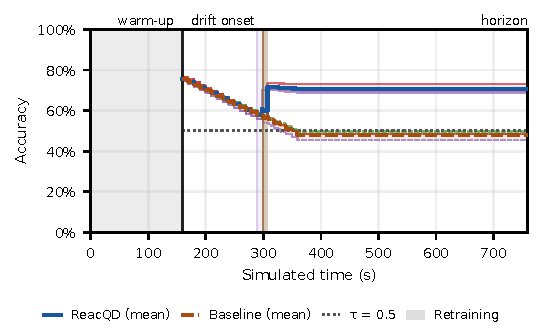
\includegraphics[width=\linewidth]{figures/fig_fog_ramp20_traj.pdf}
\caption{Fog, rampa de 200\,s, cinco seeds pareadas. Acurácia sob degradação ao
longo do tempo simulado (sólida: reativo, tracejada: baseline; linhas grossas: médias);
$\tau=0{,}5$ tracejada; faixas sombreadas: a rodada de retreinamento. A variante reativa nunca cai abaixo de $\tau$ (downtime zero).}
\label{fig:fog}
\end{figure}

\subsection{Análise do quórum coletivo}
\emph{Todos} os 10 clientes emitem alarme em cada episódio detectado (59 de 59): os detectores locais são independentes. O disparo ocorre no mínimo do quórum (0,30, três clientes distintos na janela de dois passos) em 21 de 59 episódios; o ruído Gaussiano dispara no mínimo em todos os episódios detectados da rampa de 100\,s. A rampa longa espalha os alarmes, e a fração sinalizada na decisão cai com a duração da rampa (fog $0{,}88\rightarrow0{,}42$, frosted-glass $0{,}90\rightarrow0{,}56$, motion blur $0{,}66\rightarrow0{,}54$).

\textbf{Sensibilidade a quórum e janela.} Com quórum 0,50, a política dispara em 59 de 60 episódios, deixando de detectar a mesma seed de ruído Gaussiano que com o quórum padrão 0,30 (em rampa diferente). No quórum padrão, uma janela de um passo dá resultado neutro no cômputo geral ($+3{,}7$\,s de atraso, $-3{,}9$\,s de downtime), com o sinal da diferença variando por grupo; a união de dois passos não mostra benefício sistemático.

\textbf{Staggered drift.} Quando os clientes sofrem drift em passos diferentes (cliente $i$ sofre drift no passo de operação $i$, sem rampa; 20 episódios), o gatilho coletivo dispara em 20 de 20 episódios no limiar do quórum (fração sinalizada 0,30--0,40). A política evita cerca de 81\% do downtime da baseline (600\,s, drift permanente) em três das quatro degradações e 70\% no ruído Gaussiano (116\,s e 180\,s de downtime na variante reativa, respectivamente); como o drift é instantâneo e permanente, atraso converte-se em downtime um para um (116 $\approx$ 108 + 8\,s).

\subsection{Taxa de falsos positivos em fluxos sem drift}
Executamos 15 episódios de controle (cinco seeds vezes três cronogramas de rampa) sem degradação. Cada cliente monitora um fluxo limpo pelo horizonte completo de 600\,s. O gatilho coletivo nunca dispara---nenhum dos 15 episódios registra uma decisão de retreinamento---e os detectores locais emitem zero alarmes nas 9\,000 avaliações cliente-passo. Ocorrem oito picos isolados de entropia (valores acima de 1,0), mas o ADWIN não sinaliza nenhum, pois o teste é de mudança na distribuição, não de picos. O gatilho é, assim, silencioso em fluxos sem drift e sensível sob drift (59 de 60 episódios; taxa de falsos positivos medida de 0,0\%).

\subsection{Clean retention e comportamento de recuperação}
\begin{table}[!t]
\centering
\caption{Clean retention $\Delta$ (variante reativa; média por grupo $\pm$ desvio-padrão sobre 5 seeds).}
\label{tab:retention}
\resizebox{\columnwidth}{!}{%
\begin{tabular}{lccc}
\toprule
 & \multicolumn{3}{c}{Duração da rampa}\\
\cmidrule(lr){2-4}
Degradação & 50\,s & 100\,s & 200\,s\\
\midrule
Fog & $-0{,}096\pm0{,}012$ & $-0{,}094\pm0{,}014$ & $-0{,}014\pm0{,}005$\\
Frosted-glass & $-0{,}152\pm0{,}008$ & $-0{,}156\pm0{,}014$ & $-0{,}022\pm0{,}005$\\
Motion blur & $-0{,}199\pm0{,}017$ & $-0{,}208\pm0{,}020$ & $-0{,}016\pm0{,}002$\\
Ruído Gaussiano & $-0{,}084\pm0{,}013$ & $-0{,}066\pm0{,}034$ & $-0{,}072\pm0{,}016$\\
\bottomrule
\end{tabular}}
\end{table}

Primeiro, \emph{rampas longas preservam a acurácia no conjunto limpo} (Tabela~\ref{tab:retention}). Com rampa de 200\,s, o conjunto de retreinamento mantém cerca de 30\% de dados limpos e a perda de acurácia limpa cai para 1--2 pontos (contra 9--21 em rampas curtas) para fog, frosted-glass e motion blur; o ruído Gaussiano não se beneficia (progresso do drift de 0,97 no disparo). Segundo, \emph{a recuperação não é temporária}, pois nenhum episódio volta a cruzar $\tau$ dentro do horizonte; o modelo retreinado generaliza para o regime totalmente degradado. Em 9 dos 20 episódios com rampa de 200\,s (todas as cinco execuções de fog, três de frosted-glass e uma de motion blur), a acurácia nunca cai abaixo de $\tau$. A acurácia final média por grupo, no regime totalmente degradado, varia de 0,60 a 0,71 para a variante reativa (exceto no episódio com falha, cuja acurácia final é 0,33) e de 0,35 a 0,48 para a baseline (Fig.~\ref{fig:motion}).

\begin{figure}[!t]
\centering
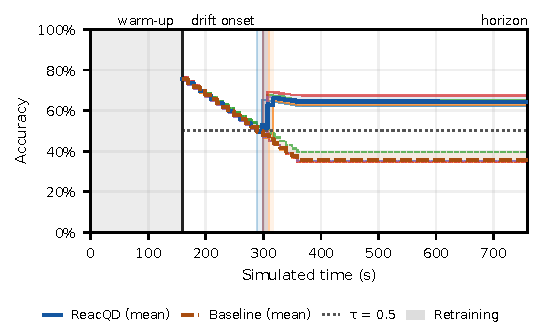
\includegraphics[width=\linewidth]{figures/fig_motion_ramp20_traj.pdf}
\caption{Motion blur, rampa de 200\,s, cinco seeds pareadas. A variante reativa recupera-se em uma rodada e permanece acima de $\tau$ durante a maior parte do horizonte; a baseline segue caindo até cerca de 0,35.}
\label{fig:motion}
\end{figure}

\section{Discussão}
O monitoramento não é gratuito. Ao longo do episódio de 80 passos (60 de operação mais 20 de warm-up), o detector com $T=5$ custa cerca de 6,8\,TFLOPs (4\,000 forward passes em lote de 32, 50 por passo nos dez clientes) contra cerca de 8,0\,TFLOPs da rodada única de retreinamento. A razão é de 0,85--0,96 conforme a contabilização, ou seja, o monitoramento responde por cerca de 47\% da computação reativa. Nos dez clientes, o monitor por passo ocupa cerca de 0,13\,s, 1,3\% de cada passo de 10\,s; no dispositivo medido uma atualização do detector leva cerca de 12,7\,ms por cliente. Se tivéssemos mantido a configuração publicada do UDD com $T=50$, o monitoramento excederia a rodada de retreinamento em cerca de $9\times$, razão pela qual a adoção de $T=5$ foi uma decisão de custo.

As conclusões sobre o downtime são robustas a uma rodada $10\times$ mais longa: ao recalcular-se o downtime \emph{a posteriori} a partir das séries registradas---atribuindo a acurácia pré-retreinamento ao intervalo $[t_d,t_d+d]$, usando o primeiro registro pós-retreinamento em diante e aplicando a regra de orçamento---, verifica-se que uma rodada de 80\,s ainda corta o downtime médio de 507,5\,s (baseline) para 122,2\,s (76\%). A ordenação por grupo, o caso de downtime zero no fog e o comportamento limitado pela detecção no ruído Gaussiano permanecem inalterados; o custo extra é exatamente o intervalo pré-retreinamento que a rodada alonga. Com $d=800$\,s, a rodada já não cabe no horizonte de operação de 600\,s e a regra de orçamento pularia o retreinamento em todos os 59 episódios em que houve disparo, de modo que a política reativa passaria a equivaler à baseline por força da regra de orçamento, e não por dinâmica de treinamento; o ponto de virada é a menor folga entre disparo e horizonte, cerca de 140\,s nesta grade.

\subsection{Ruído Gaussiano é o cenário limitante}
O ruído Gaussiano é o único cenário com detecção incompleta. Com rampa de 100\,s e seed 42, a política nunca dispara, pois só quatro dos dez clientes emitem alarme em todo o episódio, nunca três dentro da mesma janela de dois passos (fração máxima sinalizada de 0,20 em passos esparsos); as outras quatro seeds detectam em 120--210\,s. Como a janela e o quórum são idênticos entre seeds, a falha é mais bem explicada como perda do detector por cliente. Sem decisão, a variante reativa equivale exatamente à baseline (downtime de 540\,s). Com rampa de 200\,s os atrasos variam entre 180 e 460\,s (desvio-padrão de 104\,s), mas a variante reativa ainda corta o downtime da baseline em 75\% (112 vs.\ 448\,s), em consonância com o risco que detectores do tipo ADWIN carregam sob drifts longos e suaves \cite{poenaru2022}. O ruído Gaussiano é também o cenário de maior latência reativa. A Fig.~\ref{fig:gaussian} mostra a seed que falhou.

\begin{figure}[!t]
\centering
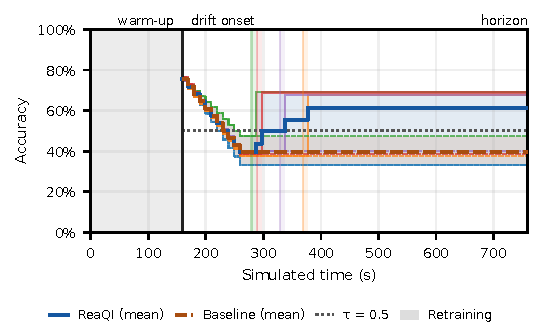
\includegraphics[width=\linewidth]{figures/fig_gaussian_ramp10_traj.pdf}
\caption{Ruído Gaussiano, rampa de 100\,s, cinco seeds pareadas. A seed 42 nunca dispara. Sua trajetória (azul sólida) não se recupera, enquanto as outras quatro seeds se recuperam para cerca de 0,68.}
\label{fig:gaussian}
\end{figure}

\subsection{Por que a rampa longa se comporta melhor}
Para as degradações visuais, a rampa de 200\,s tem três efeitos favoráveis. (i) O disparo ocorre no meio da rampa, com progresso do drift de 0,68--0,70, em que a acurácia na decisão é 0,57 para fog (ainda acima de $\tau$), 0,51 para frosted-glass e 0,48 para motion blur. (ii) O conjunto de retreinamento contém cerca de 30\% de dados limpos, reduzindo o esquecimento catastrófico. (iii) O modelo retreinado com progresso do drift de $\approx$0,7 generaliza para o regime totalmente degradado, de modo que a recuperação se sustenta. Rampas curtas comportam-se como o regime abrupto: a detecção termina após a rampa e o conjunto de retreinamento fica quase totalmente degradado. O ruído Gaussiano dispara mais tarde (progresso 0,97) e não usufrui dos efeitos (i) e (ii).

\subsection{Limitações}
Nossos resultados são limitados pelas seguintes restrições declaradas. (i) Cinco seeds por grupo limitam a precisão da estimativa de dispersão. (ii) O modelo é uma CNN pequena de cerca de 2,2 milhões de parâmetros; as acurácias absolutas sob degradação são modestas, como esperado para arquiteturas pequenas \cite{hendrycks2019}. (iii) O cenário pressupõe um único drift, uma rodada de retreinamento, partição IID, velocidade uniforme e horizonte fixo. (iv) O progresso do drift no disparo só é informativo na rampa de 200\,s. (v) O UDD publicado usa $T=50$ forward passes; o nosso $T=5$ reduz o orçamento de monitoramento por uma questão de custo, e a comparação direta entre as duas configurações não foi investigada aqui, permanecendo como trabalho futuro; $\delta=0{,}002$ é o valor padrão da implementação de referência, e não um valor calibrado \cite{baier2023,poenaru2022}. (vi) O downtime é amostrado na granularidade do passo mais o instante de conclusão da rodada. (vii) A proteção contra falsos positivos que o quórum oferece não pôde ser quantificada, de modo que nossas afirmações restringem-se à sua viabilidade e à taxa nula de falsos positivos em fluxos sem drift. Comparadores com agendamento, do tipo oráculo e com detector centralizado permanecem como trabalhos futuros. (viii) Episódios de controle sem drift (15) não produziram nenhum disparo falso (0/15), de modo que a taxa de falsos positivos do detector sob monitoramento contínuo é de 0\% nesta configuração.
\section{Conclusão e Trabalhos Futuros}
Propomos e caracterizamos uma política de decisão coletiva por quórum para o retreinamento reativo em aprendizado federado síncrono sob drift gradual: cada cliente monitora seu fluxo sem rótulos e o servidor só dispara o retreinamento quando a corroboração de clientes distintos atinge o quórum em uma janela de passos. Avaliamos a política contra uma baseline pareada sem retreinamento em 60 episódios, com downtime de serviço como métrica primária. A detecção teve êxito em 59 de 60 episódios, com o atraso crescendo com a duração da rampa para as degradações visuais; a variante reativa reduziu o downtime médio de 408--562\,s para 0--178\,s (zero no caso de fog com rampa de 200\,s); e rampas longas preservaram a acurácia limpa para as degradações visuais. O gatilho coletivo dispara nos 20 episódios de staggered drift (70--81\% do downtime da baseline evitado) com taxa de falsos positivos de 0\% em 15 controles sem drift. Trabalhos futuros incluem baselines com detector centralizado, do tipo oráculo e cientes do agendamento; mais seeds e análise formal de dispersão; drift recorrente; partições não IID; drift incremental; modelos maiores; sensibilidade aos parâmetros $T$, $\delta$ e limites de calibração do detector.

\section*{Disponibilidade}
A implementação e todos os artefatos---os 60 episódios pareados, variantes comparadoras, resumos agregados e tabelas por seed---estão disponíveis em \url{https://github.com/julio-amaral-oliveira/FederatedLearningSimulation}.
\begin{thebibliography}{29}
\bibitem{mcmahan2017} B.~McMahan, E.~Moore, D.~Ramage, S.~Hampson, and
B.~Ag{\"u}era y Arcas, ``Communication-efficient learning of deep networks
from decentralized data,'' in \emph{Proc. AISTATS}, PMLR 54,
pp.~1273--1282, 2017.
\bibitem{casado2022} F.~E. Casado, D.~Lema, M.~F. Criado, R.~Iglesias,
C.~V. Regueiro, and S.~Barro, ``Concept drift detection and adaptation for
federated and continual learning,'' \emph{Multimedia Tools and
Applications}, vol.~81, pp.~3397--3419, 2022.
\bibitem{cerqueira2026} V.~Cerqueira, H.~M. Gomes, M.~Heyden,
B.~Pfahringer, and A.~Bifet, ``A framework for evaluating and benchmarking
concept drift detection methods,'' in \emph{Proc. KDD}, 2026,
doi: 10.1145/3770855.3819070.
\bibitem{jothimurugesan2023} E.~Jothimurugesan, K.~Hsieh, J.~Wang,
G.~Joshi, and P.~B. Gibbons, ``Federated learning under distributed concept
drift,'' in \emph{Proc. AISTATS}, PMLR 206, pp.~5834--5853, 2023.
\bibitem{chow2023} T.~Chow, U.~Raza, I.~Mavromatis, and A.~Khan, ``FLARE:
Detection and mitigation of concept drift for federated learning based IoT
deployments,'' in \emph{Proc. IEEE IWCMC}, pp.~989--995, 2023.
\bibitem{mavromatis2024} I.~Mavromatis, S.~De~Feo, and A.~Khan, ``FLAME:
Adaptive and reactive concept drift mitigation for federated learning
deployments,'' arXiv:2410.01386, 2024.
\bibitem{patel2026} A.~Patel, D.~S. Tomar, R.~K. Pateriya, and
R.~Haripriya, ``FL-MalDrift: A federated learning framework for malware
detection under local concept drift,'' \emph{Scientific Reports},
vol.~16, Art.~1821, 2026.
\bibitem{han2026} Y.~Han, D.~Wu, and B.~Varghese, ``DriftGuard: Mitigating
asynchronous data drift in federated learning,'' arXiv:2603.18872, 2026.
\bibitem{fu2025} P.~Fu and M.~Tang, ``FedDAA: Dynamic client clustering for
concept drift adaptation in federated learning,'' arXiv:2506.21054, 2025.
\bibitem{zhou2026} Q.~Zhou \emph{et al.}, ``FedPLC: Federated learning with
dynamic cluster adaptation for concept drift on non-IID data,''
\emph{Sensors}, vol.~26, no.~1, Art.~283, 2026.
\bibitem{baier2023} L.~Baier, T.~Schl{\"o}r, J.~Sch{\"o}ffer, and N.~K{\"u}hl,
``Detecting concept drift with neural network model uncertainty,'' in
\emph{Proc. 56th Hawaii Int. Conf. on System Sciences (HICSS)},
pp.~835--844, 2023.
\bibitem{gal2016} Y.~Gal and Z.~Ghahramani, ``Dropout as a Bayesian
approximation: Representing model uncertainty in deep learning,'' in
\emph{Proc. ICML}, PMLR 48, pp.~1050--1059, 2016.
\bibitem{bifet2007} A.~Bifet and R.~Gavald{\`a}, ``Learning from
time-changing data with adaptive windowing,'' in \emph{Proc. SIAM Int.
Conf. on Data Mining}, pp.~443--448, 2007.
\bibitem{lobo2023} J.~L. Lobo, I.~La{\~n}a, E.~Osaba, and J.~Del~Ser, ``On
the connection between concept drift and uncertainty in industrial
artificial intelligence,'' in \emph{Proc. IEEE CAI}, pp.~171--172, 2023.
\bibitem{ovadia2019} Y.~Ovadia \emph{et al.}, ``Can you trust your model's
uncertainty? Evaluating predictive uncertainty under dataset shift,'' in
\emph{Proc. NeurIPS}, pp.~13991--14002, 2019.
\bibitem{nguyen2025} V.~Nguyen, C.~Shui, V.~Giri, S.~Arya, A.~Verma,
F.~Razak, and R.~G. Krishnan, ``Reliably detecting model failures in
deployment without labels (D3M),'' in \emph{Proc. NeurIPS}, 2025.
\bibitem{solozobov2026} O.~Solozobov, ``Label-free detection of governance
evidence degradation in risk decision systems,'' arXiv:2604.17836, 2026.
\bibitem{poenaru2022} L.~Poenaru-Olaru, L.~Cruz, A.~van~Deursen, and
J.~S. Rellermeyer, ``Are concept drift detectors reliable alarming
systems?'' arXiv:2211.13098, 2022.
\bibitem{mahdi2025} O.~A. Mahdi, E.~Pardede, S.~Bevinakoppa, and N.~Ali,
``Federated learning under concept drift: A systematic survey of
foundations, innovations, and future research directions,''
\emph{Electronics}, vol.~14, no.~22, Art.~4480, 2025.
\bibitem{bother2025} M.~B{\"o}ther \emph{et al.}, ``Modyn: Data-centric
machine learning pipeline orchestration,'' \emph{Proc. ACM on Management of
Data}, vol.~3, no.~1, Art.~55, 2025.
\bibitem{criado2022} M.~F. Criado, F.~E. Casado, R.~Iglesias, C.~V.
Regueiro, and S.~Barro, ``Non-IID data and continual learning processes in
federated learning: A long road ahead,'' \emph{Information Fusion},
vol.~88, pp.~263--280, 2022.
\bibitem{hendrycks2019} D.~Hendrycks and T.~Dietterich, ``Benchmarking
neural network robustness to common corruptions and perturbations,'' in
\emph{Proc. ICLR}, 2019.
\bibitem{panchal2023} K.~Panchal \emph{et al.}, ``Flash: Concept drift
adaptation in federated learning,'' in \emph{Proc. ICML}, PMLR 202,
pp.~26931--26962, 2023.
\bibitem{chen2026} X.~Chen \emph{et al.}, ``Virtual concept drift detection
and adaptation in federated data stream learning,'' \emph{Int.\ J.\ Data
Science and Analytics}, vol.~21, Art.~46, 2026.
\bibitem{stallmann2024} M.~Stallmann, A.~Wilbik, and G.~Wei{\ss}, ``Towards
unsupervised sudden data drift detection in federated learning with fuzzy
clustering,'' in \emph{Proc. IEEE FUZZ-IEEE}, 2024.
\bibitem{bhope2025} R.~A. Bhope, K.~R. Jayaram, P.~Venkateswaran, and
N.~Venkatasubramanian, ``Shift happens: Mixture of experts based continual
adaptation in federated learning,'' in \emph{Proc. ACM Middleware},
pp.~455--468, 2025.
\bibitem{canonaco2021} G.~Canonaco, A.~Bergamasco, A.~Mongelluzzo, and
M.~Roveri, ``Adaptive federated learning in presence of concept drift,'' in
\emph{Proc. IEEE Int. Joint Conf. on Neural Networks (IJCNN)},
pp.~1--7, 2021.
\bibitem{lu2025} P.~Lu, J.~Lu, A.~Liu, and G.~Zhang, ``Early concept drift
detection via prediction uncertainty,'' in \emph{Proc. AAAI Conf. on
Artificial Intelligence}, vol.~39, no.~18, pp.~19124--19132, 2025.
\bibitem{zhang2025} B.~Zhang, H.~Guan, H.~K. Lee, R.~Liu, J.~Zou, and
L.~Xiong, ``FedSGT: Exact federated unlearning via sequential group-based
training,'' arXiv:2511.23393, 2025.
\end{thebibliography}

\end{document}
